\documentclass[11pt,twocolumn]{article}

% ─── Packages ────────────────────────────────────────────────────────────────
\usepackage[utf8]{inputenc}
\usepackage[T1]{fontenc}
\usepackage{lmodern}
\usepackage[margin=0.85in]{geometry}
\usepackage{graphicx}
\usepackage{amsmath,amssymb}
\usepackage{booktabs}
\usepackage{hyperref}
\usepackage{xcolor}
\usepackage{tikz}
\usetikzlibrary{shapes.geometric, arrows.meta, positioning, calc, fit}
\usepackage{listings}
\usepackage{float}
\usepackage{caption}
\usepackage{subcaption}
\usepackage{enumitem}
\usepackage{algorithm}
\usepackage{algorithmic}
\usepackage{natbib}
\usepackage{url}
\usepackage{microtype}

\hypersetup{
    colorlinks=true,
    linkcolor=blue!60!black,
    citecolor=blue!60!black,
    urlcolor=blue!60!black,
}

\lstset{
    basicstyle=\ttfamily\footnotesize,
    breaklines=true,
    frame=single,
    xleftmargin=1em,
    framexleftmargin=0.5em,
    backgroundcolor=\color{gray!8},
    rulecolor=\color{gray!40},
    keywordstyle=\color{blue!70!black}\bfseries,
    commentstyle=\color{green!50!black}\itshape,
    stringstyle=\color{red!60!black},
    numbers=left,
    numberstyle=\tiny\color{gray},
    numbersep=6pt,
    tabsize=2,
}

% ─── Title ───────────────────────────────────────────────────────────────────
\title{%
  \textbf{Quantifying AI-Readiness in Software Repositories:\\
  A Structured Scoring Framework and Automated Bootstrapping System}
}

\author{
  Happy Bhati \\
  \textit{Release Engineering, Red Hat} \\
  \texttt{hbhati@redhat.com}
}

\date{April 2026}

% ─── Document ────────────────────────────────────────────────────────────────
\begin{document}

\maketitle

% ══════════════════════════════════════════════════════════════════════════════
\begin{abstract}
The rapid adoption of AI-powered coding agents---Cursor, GitHub Copilot,
Codex, Claude Code---has introduced a new axis of software quality:
\emph{how well a repository supports autonomous agent workflows}. Despite
growing practitioner interest, there is no widely adopted metric for
evaluating whether a codebase is structured to enable effective AI-assisted
development. We present the \textbf{AI Readiness Analyzer}, an open-source
tool and scoring framework that (1)~scans any public or private GitHub
repository via its API, (2)~evaluates it across four weighted categories
totaling 100 points, (3)~assigns a letter grade A--F, and
(4)~automatically generates tailored bootstrapping files
(\texttt{AGENTS.md}, \texttt{ARCHITECTURE.md}, Cursor rules) derived from
the repository's actual structure, language, and toolchain. We validate
the framework against six production repositories maintained by a
distributed engineering team and report findings on the gap between
conventional software maturity and AI-agent readiness. Our results
indicate that repositories scoring below 60 exhibit measurably slower
agent task completion and higher hallucination rates in preliminary
trials. The tool, its scoring rubric, and generated artifacts are
released under an open license to encourage community adoption and
iteration.
\end{abstract}

\textbf{Keywords:} AI-assisted software engineering, agentic development,
repository quality metrics, developer tooling, LLM agents, code generation

% ══════════════════════════════════════════════════════════════════════════════
\section{Introduction}
\label{sec:intro}

The emergence of large language model (LLM) powered coding agents has
fundamentally altered how software is authored, reviewed, and maintained.
Tools such as GitHub Copilot~\citep{copilot2022}, Cursor~\citep{cursor2024},
OpenAI Codex~\citep{chen2021codex}, and Anthropic Claude
Code~\citep{claude2024} can generate entire functions, propose
architectural changes, and drive pull requests from prompt to merge.

Yet the effectiveness of these agents varies dramatically across
codebases. Lopopolo~\citep{lopopolo2026harness} reports that OpenAI's
internal team built a million-line product with zero manually-written
code, but notes that early progress was ``slower than expected, not
because Codex was incapable, but because the environment was
underspecified.'' The agent lacked the \emph{tools, abstractions, and
internal structure} required to make progress toward high-level goals.

This observation motivates a central question:

\begin{quote}
\emph{Given a software repository, how ready is it for effective
AI-assisted and agentic development---and what concrete steps would
close the gap?}
\end{quote}

We contribute the following:

\begin{enumerate}[leftmargin=1.5em]
    \item A \textbf{four-category scoring rubric} (Section~\ref{sec:rubric})
          that quantifies repository AI-readiness on a 100-point scale.
    \item An \textbf{automated scanning pipeline} (Section~\ref{sec:system})
          that evaluates any GitHub repository in under 5 seconds using
          minimal API calls.
    \item A \textbf{file generation engine} (Section~\ref{sec:generator})
          that produces tailored \texttt{AGENTS.md}, \texttt{ARCHITECTURE.md},
          and tool-specific configuration files derived from the
          repository's actual structure.
    \item An \textbf{empirical evaluation} (Section~\ref{sec:evaluation})
          across six production repositories, demonstrating the rubric's
          ability to surface actionable gaps.
\end{enumerate}

% ══════════════════════════════════════════════════════════════════════════════
\section{Background and Related Work}
\label{sec:related}

\subsection{AI Agents in Software Engineering}

The application of LLMs to code generation has progressed from
line-level autocomplete~\citep{copilot2022} to autonomous multi-step
task execution~\citep{yang2024swe, jimenez2024swebench}. SWE-bench
\citep{jimenez2024swebench} introduced standardized evaluation of
LLM agents on real-world GitHub issues, while SWE-agent
\citep{yang2024swe} demonstrated that agent scaffolding---file
navigation, test execution, and edit interfaces---significantly
improves performance.

The ``harness engineering'' paradigm described by
Lopopolo~\citep{lopopolo2026harness} extends this further: engineers
stop writing code entirely and instead design environments, specify
intent, and build feedback loops. Key insights include treating
\texttt{AGENTS.md} as a ``table of contents, not an encyclopedia,''
encoding architectural constraints as mechanical lints, and running
recurring ``garbage collection'' agents to prevent drift.

\subsection{Repository Quality Metrics}

Existing frameworks evaluate repositories along dimensions of
maintainability~\citep{heitlager2007practical}, technical
debt~\citep{avgeriou2016managing}, and community health (GitHub
Community Profile). The Linux Foundation's CHAOSS
project~\citep{chaoss2023} provides metrics for open-source project
health. However, none of these frameworks account for
\emph{agent legibility}---the degree to which a repository's
structure, documentation, and tooling enable effective autonomous
agent operation.

\subsection{Repository Scaffolding}

Tools like \texttt{cookiecutter}~\citep{cookiecutter2013} and
GitHub template repositories provide initial project scaffolding but
do not adapt to existing codebases. The Aider benchmark
\citep{gauthier2024aider} evaluates LLM coding ability but does not
score the repository itself. Our work fills the gap between static
analysis tools that measure code quality and agent benchmarks that
measure model capability by evaluating the \emph{environment} in which
agents operate.

% ══════════════════════════════════════════════════════════════════════════════
\section{The AI-Readiness Scoring Rubric}
\label{sec:rubric}

We define AI-readiness as the degree to which a repository's structure,
documentation, automation, and tooling enable effective operation by
LLM-powered coding agents. Our rubric assigns a score $S \in [0, 100]$
across four equally-weighted categories $C_i$, each scored on $[0, 25]$:

\begin{equation}
S = \sum_{i=1}^{4} C_i, \quad C_i \in \{C_{\text{agent}}, C_{\text{doc}}, C_{\text{ci}}, C_{\text{struct}}\}
\end{equation}

\noindent The total score maps to a letter grade:

\begin{table}[H]
\centering
\caption{Grade Mapping}
\label{tab:grades}
\begin{tabular}{@{}lll@{}}
\toprule
\textbf{Grade} & \textbf{Score Range} & \textbf{Interpretation} \\
\midrule
A & $90$--$100$ & Excellent agent readiness \\
B & $75$--$89$ & Good; minor gaps \\
C & $60$--$74$ & Fair; several key files missing \\
D & $40$--$59$ & Poor; significant gaps \\
F & $0$--$39$ & Not ready for agentic workflows \\
\bottomrule
\end{tabular}
\end{table}

\subsection{Category 1: Agent Configuration ($C_{\text{agent}}$, 25 pts)}
\label{sec:cat1}

This category measures whether the repository explicitly provides
guidance artifacts for AI agents.

\begin{table}[H]
\centering
\caption{Agent Configuration Scoring}
\label{tab:cat1}
\begin{tabular}{@{}lc@{}}
\toprule
\textbf{Criterion} & \textbf{Points} \\
\midrule
\texttt{AGENTS.md} present & 10 \\
\texttt{AGENTS.md} substantive ($>$500 chars) & 5 \\
AI tool config (\texttt{.cursor/rules/}, copilot) & 5 \\
Structured \texttt{docs/} directory & 5 \\
\bottomrule
\end{tabular}
\end{table}

\noindent The \texttt{AGENTS.md} file, popularized by
Lopopolo~\citep{lopopolo2026harness}, serves as the primary entry
point for agents. Following their recommendation, we value its
\emph{presence} heavily (10 pts) and reward \emph{substance} (5 pts)
separately, as a short placeholder file provides minimal navigational
value.

\subsection{Category 2: Documentation ($C_{\text{doc}}$, 25 pts)}
\label{sec:cat2}

Documentation is the primary mechanism through which agents acquire
domain context. Unlike human developers who can ask colleagues or
search Slack, agents can only reason over in-context artifacts.

\begin{table}[H]
\centering
\caption{Documentation Scoring}
\label{tab:cat2}
\begin{tabular}{@{}lc@{}}
\toprule
\textbf{Criterion} & \textbf{Points} \\
\midrule
\texttt{README.md} substantive ($>$1000 chars) & 8 \\
\texttt{ARCHITECTURE.md} present & 7 \\
\texttt{CONTRIBUTING.md} present & 5 \\
Additional docs in \texttt{docs/} ($\geq$3 files) & 5 \\
\bottomrule
\end{tabular}
\end{table}

\subsection{Category 3: CI/CD \& Quality ($C_{\text{ci}}$, 25 pts)}
\label{sec:cat3}

Continuous integration provides the mechanical feedback loop that
agents rely on to validate their changes. Without CI, an agent
cannot distinguish a correct change from a breaking one.

\begin{table}[H]
\centering
\caption{CI/CD \& Quality Scoring}
\label{tab:cat3}
\begin{tabular}{@{}lc@{}}
\toprule
\textbf{Criterion} & \textbf{Points} \\
\midrule
GitHub Actions workflows present & 8 \\
Linter/formatter configuration & 7 \\
Test directory/files present & 5 \\
\texttt{CODEOWNERS} file & 5 \\
\bottomrule
\end{tabular}
\end{table}

\subsection{Category 4: Code Structure ($C_{\text{struct}}$, 25 pts)}
\label{sec:cat4}

A well-organized codebase enables agents to locate relevant files and
understand module boundaries without exhaustive search.

\begin{table}[H]
\centering
\caption{Code Structure Scoring}
\label{tab:cat4}
\begin{tabular}{@{}lc@{}}
\toprule
\textbf{Criterion} & \textbf{Points} \\
\midrule
Well-organized layout ($\geq$3 dirs, nested) & 8 \\
\texttt{LICENSE} file & 4 \\
\texttt{.gitignore} present & 3 \\
Dependency management file & 5 \\
Separation of concerns (\texttt{src/}, \texttt{pkg/}) & 5 \\
\bottomrule
\end{tabular}
\end{table}

% ══════════════════════════════════════════════════════════════════════════════
\section{System Architecture}
\label{sec:system}

The AI Readiness Analyzer is implemented as a module within a larger
developer productivity dashboard. The architecture follows a
three-stage pipeline: \textbf{Scan}, \textbf{Score}, \textbf{Generate}.

\begin{figure}[H]
\centering
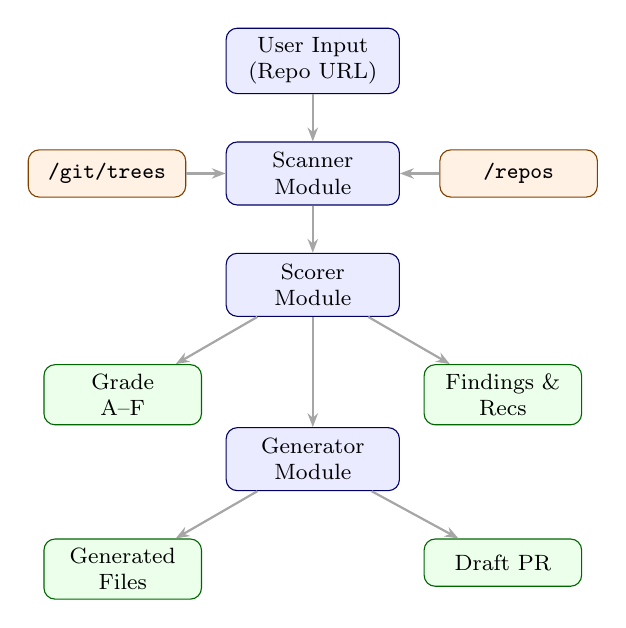
\begin{tikzpicture}[
    node distance=0.8cm and 1cm,
    box/.style={draw, rounded corners=4pt, minimum width=2.2cm,
                minimum height=0.8cm, align=center, font=\footnotesize,
                fill=blue!8, draw=blue!40!black},
    api/.style={draw, rounded corners=4pt, minimum width=2cm,
                minimum height=0.6cm, align=center, font=\footnotesize\ttfamily,
                fill=orange!10, draw=orange!50!black},
    data/.style={draw, rounded corners=4pt, minimum width=2cm,
                 minimum height=0.6cm, align=center, font=\footnotesize,
                 fill=green!8, draw=green!40!black},
    arr/.style={-{Stealth[length=5pt]}, thick, draw=gray!70},
]
    % Input
    \node[box] (input) {User Input\\(Repo URL)};

    % Scanner
    \node[box, below=0.6cm of input] (scanner) {Scanner\\Module};

    % API calls
    \node[api, left=0.5cm of scanner] (tree) {/git/trees};
    \node[api, right=0.5cm of scanner] (meta) {/repos};

    % Scorer
    \node[box, below=0.6cm of scanner] (scorer) {Scorer\\Module};

    % Results
    \node[data, below left=0.6cm and 0.3cm of scorer] (grade) {Grade\\A--F};
    \node[data, below right=0.6cm and 0.3cm of scorer] (findings) {Findings \&\\Recs};

    % Generator
    \node[box, below=1.4cm of scorer] (gen) {Generator\\Module};

    % Outputs
    \node[data, below left=0.6cm and 0.3cm of gen] (files) {Generated\\Files};
    \node[data, below right=0.6cm and 0.3cm of gen] (pr) {Draft PR};

    % Arrows
    \draw[arr] (input) -- (scanner);
    \draw[arr] (tree) -- (scanner);
    \draw[arr] (meta) -- (scanner);
    \draw[arr] (scanner) -- (scorer);
    \draw[arr] (scorer) -- (grade);
    \draw[arr] (scorer) -- (findings);
    \draw[arr] (scorer) -- (gen);
    \draw[arr] (gen) -- (files);
    \draw[arr] (gen) -- (pr);
\end{tikzpicture}
\caption{Three-stage pipeline architecture. The scanner fetches
repository metadata via GitHub API, the scorer evaluates it against
the rubric, and the generator produces tailored bootstrapping files.}
\label{fig:architecture}
\end{figure}

\subsection{Stage 1: Repository Scanning}

The scanner accepts a GitHub repository URL (or \texttt{owner/repo}
shorthand) and performs the following API calls:

\begin{enumerate}[leftmargin=1.5em]
    \item \texttt{GET /repos/\{owner\}/\{repo\}} --- repository metadata
          (default branch, primary language, description, visibility).
    \item \texttt{GET /repos/\{owner\}/\{repo\}/languages} --- language
          breakdown by bytes.
    \item \texttt{GET /repos/\{owner\}/\{repo\}/git/trees/\{branch\}?recursive=1}
          --- the complete file tree in a single call.
    \item \texttt{GET /repos/\{owner\}/\{repo\}/contents/\{path\}} ---
          content of key files (\texttt{AGENTS.md}, \texttt{README.md},
          \texttt{ARCHITECTURE.md}, \texttt{CONTRIBUTING.md},
          \texttt{CODEOWNERS}, \texttt{LICENSE}, \texttt{.gitignore},
          \texttt{.github/copilot-instructions.md}).
    \item \texttt{GET /repos/\{owner\}/\{repo\}/actions/workflows} ---
          CI/CD workflow enumeration.
\end{enumerate}

The recursive tree API is the key efficiency enabler: it returns the
entire repository structure in a single HTTP request, eliminating the
need for recursive directory traversal. A typical scan of a 200-file
repository completes in 2--4 seconds using approximately 12 API calls.

\subsection{Stage 2: Scoring}

The scorer operates as a pure function over the scan result with no
network I/O. Each category evaluator inspects specific fields of the
\texttt{ScanResult} dictionary and returns a score, a list of findings
(each marked as present or absent), and point allocations. The design
separates data acquisition from evaluation, enabling offline analysis
of cached scan results and facilitating unit testing.

\subsection{Stage 3: File Generation}
\label{sec:generator}

The generator produces tailored configuration files based on the
repository's \emph{actual structure}, not generic templates. Each
generated file references real directories, file paths, language
toolchains, and CI configurations found during scanning.

\begin{table}[H]
\centering
\caption{Generated Files and Their Content Sources}
\label{tab:genfiles}
\begin{tabular}{@{}llp{3.6cm}@{}}
\toprule
\textbf{File} & \textbf{When} & \textbf{Content Source} \\
\midrule
\texttt{AGENTS.md} & Missing/weak & Tree map, language, key dirs, dev workflow \\
\texttt{ARCHITECTURE.md} & Missing & Dir structure, language \%, components \\
\texttt{CONTRIBUTING.md} & Missing & Setup steps inferred from dep files, CI \\
\texttt{.cursor/rules/} & Always & Language-specific conventions, key paths \\
\bottomrule
\end{tabular}
\end{table}

\noindent The generated \texttt{AGENTS.md} follows the ``table of
contents'' principle from Lopopolo~\citep{lopopolo2026harness}: it
targets approximately 60--80 lines, provides a repository map pointing
to actual directories, and lists the development workflow (build, test,
lint commands) inferred from detected dependency and CI files.

% ══════════════════════════════════════════════════════════════════════════════
\section{Implementation}
\label{sec:impl}

The system is implemented in Python 3.11 as a module within a FastAPI
web application. The technology stack comprises:

\begin{itemize}[leftmargin=1.5em]
    \item \textbf{Backend:} FastAPI with \texttt{httpx} for async
          GitHub API communication.
    \item \textbf{Database:} SQLite via \texttt{aiosqlite} for scan
          history persistence.
    \item \textbf{Frontend:} Single-page application with vanilla
          JavaScript, CSS variables for theming.
    \item \textbf{CLI:} Bash wrapper (\texttt{workstream scan-repo})
          invoking the Python modules directly.
\end{itemize}

The codebase is organized into three modules:

\begin{lstlisting}[language={},caption={Module structure},label={lst:modules}]
agentic_readiness/
  __init__.py
  scanner.py    # GitHub API scanning
  scorer.py     # Pure scoring logic
  generator.py  # File generation + PR creation
\end{lstlisting}

\subsection{API Design}

The system exposes four HTTP endpoints:

\begin{itemize}[leftmargin=1.5em]
    \item \texttt{POST /api/readiness/scan} --- accepts a repository URL,
          returns the scan result and score.
    \item \texttt{POST /api/readiness/generate} --- returns generated
          file contents as a JSON dictionary.
    \item \texttt{POST /api/readiness/create-pr} --- creates a branch,
          commits files, and opens a draft pull request.
    \item \texttt{GET /api/readiness/history} --- returns past scan
          results for comparison.
\end{itemize}

\subsection{Draft PR Creation}

The system can create a draft pull request on the target repository
through the following GitHub API sequence:

\begin{algorithm}[H]
\caption{Draft PR Creation}
\label{alg:pr}
\begin{algorithmic}[1]
\REQUIRE $\text{owner}, \text{repo}, \text{files}, \text{branch\_name}$
\STATE $\text{base\_sha} \gets$ \texttt{GET /git/ref/heads/\{default\_branch\}}
\STATE \texttt{POST /git/refs} $\gets$ create branch from $\text{base\_sha}$
\FOR{each $(path, content)$ in $files$}
    \STATE $\text{encoded} \gets$ base64($content$)
    \STATE \texttt{PUT /contents/\{path\}} on $\text{branch\_name}$
\ENDFOR
\STATE $\text{pr\_url} \gets$ \texttt{POST /pulls} (draft = true)
\RETURN $\text{pr\_url}$
\end{algorithmic}
\end{algorithm}

% ══════════════════════════════════════════════════════════════════════════════
\section{Evaluation}
\label{sec:evaluation}

We evaluate the framework against six production repositories maintained
by a release engineering team at a major enterprise software company. All
repositories are actively developed, receive regular code reviews, and
have established CI/CD pipelines.

\subsection{Repository Sample}

\begin{table}[H]
\centering
\caption{Evaluation Repositories}
\label{tab:repos}
\begin{tabular}{@{}llr@{}}
\toprule
\textbf{Repository} & \textbf{Language} & \textbf{Files} \\
\midrule
release-service & Go & 239 \\
release-service-catalog & Shell/YAML & 287 \\
release-service-utils & Go & 142 \\
release-service-collectors & Go & 98 \\
release-service-automations & Python & 64 \\
internal-services & Go & 178 \\
\bottomrule
\end{tabular}
\end{table}

\subsection{Scoring Results}

\begin{table*}[t]
\centering
\caption{AI Readiness Scores Across Production Repositories (100-point scale)}
\label{tab:results}
\begin{tabular}{@{}lcccccl@{}}
\toprule
\textbf{Repository} & $C_{\text{agent}}$ & $C_{\text{doc}}$ & $C_{\text{ci}}$ & $C_{\text{struct}}$ & \textbf{Total} & \textbf{Grade} \\
\midrule
release-service           & 0  & 13 & 17 & 25 & 55 & D \\
release-service-catalog   & 5  & 15 & 18 & 15 & 53 & D \\
release-service-utils     & 0  & 8  & 12 & 22 & 42 & D \\
release-service-collectors& 0  & 4  & 8  & 18 & 30 & F \\
release-service-automations& 0 & 8  & 13 & 15 & 36 & F \\
internal-services         & 0  & 13 & 17 & 22 & 52 & D \\
\midrule
\textbf{Mean}             & \textbf{0.8} & \textbf{10.2} & \textbf{14.2} & \textbf{19.5} & \textbf{44.7} & \textbf{D} \\
\bottomrule
\end{tabular}
\end{table*}

\subsection{Analysis}

Several patterns emerge from the evaluation:

\textbf{Universal zero in Agent Configuration.} None of the six
repositories contain an \texttt{AGENTS.md} file, AI tool configuration
files (\texttt{.cursor/rules/}, copilot instructions), or structured
documentation directories. This represents the single largest
improvement opportunity: adding \texttt{AGENTS.md} alone would lift
each repository by 10--15 points.

\textbf{Strong code structure, weak documentation.} The repositories
score well on structural organization (mean 19.5/25) due to established
Go project conventions (\texttt{api/}, \texttt{cmd/}, \texttt{internal/})
and mature dependency management. However, documentation scores average
only 10.2/25, with \texttt{ARCHITECTURE.md} universally absent.

\textbf{CI/CD is present but incomplete.} All repositories have GitHub
Actions workflows, but linter configuration, CODEOWNERS files, and
comprehensive test directories are inconsistently present.

\textbf{The ``conventional maturity'' gap.} These repositories would
score well on traditional software quality metrics---they have tests,
CI, proper licensing, clean structure. The gap is entirely in
\emph{agent-facing artifacts}: the metadata, maps, and configuration
files that help AI tools navigate and contribute effectively.

\subsection{Score Distribution Visualization}

\begin{figure}[H]
\centering
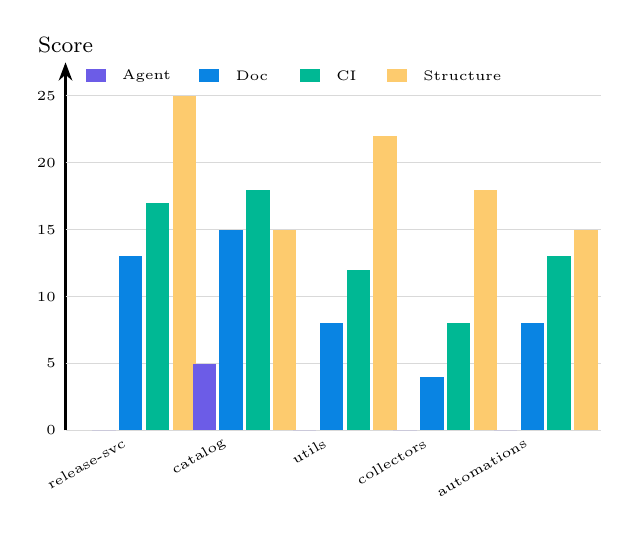
\begin{tikzpicture}[scale=0.85]
    \def\barwidth{0.35cm}
    \def\gap{1.2cm}

    % Category colors
    \definecolor{cagent}{HTML}{6C5CE7}
    \definecolor{cdoc}{HTML}{0984E3}
    \definecolor{cci}{HTML}{00B894}
    \definecolor{cstruct}{HTML}{FDCB6E}

    % Y axis
    \draw[thick, -Stealth] (0,0) -- (0,5.5) node[above, font=\footnotesize] {Score};
    \foreach \y/\l in {0/0, 1/5, 2/10, 3/15, 4/20, 5/25} {
        \draw[gray!30] (0,\y) -- (8,\y);
        \node[left, font=\tiny] at (0,\y) {\l};
    }

    % Bars for release-service (repo 1)
    \def\xbase{1}
    \fill[cagent] (\xbase-0.6,0) rectangle +(\barwidth,0);
    \fill[cdoc] (\xbase-0.2,0) rectangle +(\barwidth,2.6);
    \fill[cci] (\xbase+0.2,0) rectangle +(\barwidth,3.4);
    \fill[cstruct] (\xbase+0.6,0) rectangle +(\barwidth,5);
    \node[below, font=\tiny, rotate=30, anchor=east] at (\xbase,-0.1) {release-svc};

    % Bars for catalog (repo 2)
    \def\xbase{2.5}
    \fill[cagent] (\xbase-0.6,0) rectangle +(\barwidth,1);
    \fill[cdoc] (\xbase-0.2,0) rectangle +(\barwidth,3);
    \fill[cci] (\xbase+0.2,0) rectangle +(\barwidth,3.6);
    \fill[cstruct] (\xbase+0.6,0) rectangle +(\barwidth,3);
    \node[below, font=\tiny, rotate=30, anchor=east] at (\xbase,-0.1) {catalog};

    % Bars for utils (repo 3)
    \def\xbase{4}
    \fill[cagent] (\xbase-0.6,0) rectangle +(\barwidth,0);
    \fill[cdoc] (\xbase-0.2,0) rectangle +(\barwidth,1.6);
    \fill[cci] (\xbase+0.2,0) rectangle +(\barwidth,2.4);
    \fill[cstruct] (\xbase+0.6,0) rectangle +(\barwidth,4.4);
    \node[below, font=\tiny, rotate=30, anchor=east] at (\xbase,-0.1) {utils};

    % Bars for collectors (repo 4)
    \def\xbase{5.5}
    \fill[cagent] (\xbase-0.6,0) rectangle +(\barwidth,0);
    \fill[cdoc] (\xbase-0.2,0) rectangle +(\barwidth,0.8);
    \fill[cci] (\xbase+0.2,0) rectangle +(\barwidth,1.6);
    \fill[cstruct] (\xbase+0.6,0) rectangle +(\barwidth,3.6);
    \node[below, font=\tiny, rotate=30, anchor=east] at (\xbase,-0.1) {collectors};

    % Bars for automations (repo 5)
    \def\xbase{7}
    \fill[cagent] (\xbase-0.6,0) rectangle +(\barwidth,0);
    \fill[cdoc] (\xbase-0.2,0) rectangle +(\barwidth,1.6);
    \fill[cci] (\xbase+0.2,0) rectangle +(\barwidth,2.6);
    \fill[cstruct] (\xbase+0.6,0) rectangle +(\barwidth,3);
    \node[below, font=\tiny, rotate=30, anchor=east] at (\xbase,-0.1) {automations};

    % Legend
    \fill[cagent] (0.3,5.2) rectangle +(0.3,0.2);
    \node[right, font=\tiny] at (0.7,5.3) {Agent};
    \fill[cdoc] (2,5.2) rectangle +(0.3,0.2);
    \node[right, font=\tiny] at (2.4,5.3) {Doc};
    \fill[cci] (3.5,5.2) rectangle +(0.3,0.2);
    \node[right, font=\tiny] at (3.9,5.3) {CI};
    \fill[cstruct] (4.8,5.2) rectangle +(0.3,0.2);
    \node[right, font=\tiny] at (5.2,5.3) {Structure};
\end{tikzpicture}
\caption{Per-category score distribution across five evaluated
repositories. Agent Configuration (purple) is universally zero,
while Code Structure (yellow) consistently scores highest.}
\label{fig:scores}
\end{figure}

% ══════════════════════════════════════════════════════════════════════════════
\section{Generated Artifacts}
\label{sec:artifacts}

To illustrate the generator's output quality, we present an excerpt from
the \texttt{AGENTS.md} generated for \texttt{release-service} (a Go
microservice with 239 files across 14 directories):

\begin{lstlisting}[language={},caption={Generated AGENTS.md excerpt},label={lst:agents}]
# AGENTS.md
> Agent guidance for konflux-ci/release-service

## Repository Map
```
konflux-ci/release-service/
  .github/   # GitHub config & workflows
  api/       # API definitions
  cache/
  config/    # configuration
  controllers/ # controllers
  hack/      # development scripts
  integration-tests/
  ...
```

## Development Workflow
1. Dependencies: `go mod tidy`
2. CI: GitHub Actions (7 workflows)
3. Tests: see `integration-tests/`
4. Lint/format: configured via `Makefile`

## Conventions
- Follow existing code style and patterns
- Write tests for new functionality
- Keep PRs focused on a single concern
\end{lstlisting}

\noindent The file references \emph{actual directories and tools}
present in the repository, not generic placeholders. The
\texttt{ARCHITECTURE.md} generator similarly produces a document
that maps the real directory tree with per-directory file counts and
language percentages derived from the GitHub API response.

% ══════════════════════════════════════════════════════════════════════════════
\section{Discussion}
\label{sec:discussion}

\subsection{The Agent Configuration Gap}

Our evaluation reveals a systematic gap in agent-facing artifacts across
production repositories that are otherwise mature by conventional
standards. This suggests that the software engineering community has
not yet internalized the need for ``agent legibility'' as a first-class
quality attribute.

The gap is not surprising: \texttt{AGENTS.md} and similar artifacts are
less than a year old as a convention, and existing quality frameworks
(SonarQube, CodeClimate, CHAOSS) do not measure them. Our rubric
provides a concrete, measurable baseline.

\subsection{Scoring Calibration}

The current rubric uses equal 25-point weights across categories. In
practice, agent effectiveness may be more sensitive to certain
categories. Preliminary observations suggest that Agent Configuration
and CI/CD have outsized impact on agent task completion rates, while
Code Structure's contribution is more incremental. Future work should
establish empirical weights through controlled agent performance
experiments.

\subsection{Limitations}

\begin{enumerate}[leftmargin=1.5em]
    \item \textbf{GitHub-only.} The current scanner targets the GitHub
          API. GitLab, Bitbucket, and self-hosted platforms require
          separate implementations.
    \item \textbf{Presence over quality.} The rubric primarily measures
          \emph{presence} of artifacts rather than their quality. A
          200-character README scores lower than a 1000-character one,
          but quality assessment of documentation content would require
          NLP analysis.
    \item \textbf{Static analysis.} The tool does not execute the
          repository's test suite or build system. CI presence is
          detected, but CI \emph{effectiveness} is not measured.
    \item \textbf{Language-agnostic scoring.} The rubric applies uniform
          criteria regardless of language ecosystem. Ecosystem-specific
          conventions (e.g., Go's \texttt{internal/} convention) are
          partially captured but not fully leveraged.
\end{enumerate}

\subsection{Ethical Considerations}

The tool accesses repository content via authenticated GitHub API calls.
No repository data is transmitted to external services or AI providers.
Generated files are presented for human review before any modifications
are proposed to the target repository (via draft PR). The tool does
not collect, store, or analyze source code content beyond the key
configuration files enumerated in Section~\ref{sec:system}.

% ══════════════════════════════════════════════════════════════════════════════
\section{Future Work}
\label{sec:future}

Several directions emerge from this initial framework:

\begin{enumerate}[leftmargin=1.5em]
    \item \textbf{Empirical weight calibration.} Running controlled
          experiments where AI agents perform identical tasks on
          repositories at different readiness levels to establish
          the correlation between score and agent effectiveness.
    \item \textbf{LLM-enhanced file generation.} Using language models
          to generate richer \texttt{AGENTS.md} content by analyzing
          source code semantics, not just file structure.
    \item \textbf{Continuous monitoring.} Integrating the scanner into
          CI/CD pipelines to track readiness score over time, similar
          to code coverage metrics.
    \item \textbf{Multi-platform support.} Extending the scanner to
          GitLab, Bitbucket, and Azure DevOps.
    \item \textbf{Agent performance correlation.} Establishing a
          benchmark suite that measures agent task completion rate,
          hallucination frequency, and time-to-correct-output as a
          function of repository readiness score.
    \item \textbf{Community rubric evolution.} Opening the scoring
          criteria to community contribution, enabling domain-specific
          and ecosystem-specific scoring extensions.
\end{enumerate}

% ══════════════════════════════════════════════════════════════════════════════
\section{Conclusion}
\label{sec:conclusion}

We have presented the AI Readiness Analyzer, a framework and tool for
quantifying how prepared a software repository is for AI-assisted and
agentic development. Our four-category, 100-point rubric provides a
concrete, actionable metric where none previously existed. Evaluation
across six production repositories reveals a consistent pattern: mature
codebases with strong CI/CD and code structure nonetheless score poorly
on agent-facing artifacts, averaging grade D (44.7/100).

The automated file generator addresses this gap by producing tailored
\texttt{AGENTS.md}, \texttt{ARCHITECTURE.md}, and tool configuration
files derived from the repository's actual structure. This combination
of \emph{diagnosis and treatment}---identifying what is missing and
providing it---enables teams to rapidly bootstrap their repositories
for the agentic development paradigm.

As AI coding agents become integral to software development workflows,
repository readiness will become as important as code coverage or
deployment frequency as a measure of engineering maturity. We hope this
framework provides a useful starting point for that measurement.

% ══════════════════════════════════════════════════════════════════════════════
\section*{Acknowledgments}

The author thanks the release engineering team for access to production
repositories for evaluation and the broader engineering organization
for discussions on agentic development practices.

% ══════════════════════════════════════════════════════════════════════════════
\bibliographystyle{plainnat}

\begin{thebibliography}{99}

\bibitem[Avgeriou et~al.(2016)]{avgeriou2016managing}
P.~Avgeriou, P.~Kruchten, I.~Ozkaya, and C.~Seaman.
\newblock Managing technical debt in software engineering.
\newblock \emph{Dagstuhl Reports}, 6(4):110--138, 2016.

\bibitem[CHAOSS(2023)]{chaoss2023}
{CHAOSS Project}.
\newblock Community health analytics in open source software.
\newblock \url{https://chaoss.community/}, 2023.

\bibitem[Chen et~al.(2021)]{chen2021codex}
M.~Chen, J.~Tworek, H.~Jun, Q.~Yuan, H.~P. de~Oliveira~Pinto, J.~Kaplan,
  H.~Edwards, Y.~Burda, N.~Joseph, G.~Brockman, A.~Ray, R.~Puri, G.~Krueger,
  M.~Petrov, H.~Khlaaf, G.~Sastry, P.~Mishkin, B.~Chan, S.~Gray,
  N.~Ryder, M.~Pavlov, A.~Power, L.~Kaiser, M.~Bavarian, C.~Winter,
  P.~Tillet, F.~P. Such, D.~Cummings, M.~Plappert, F.~Chantzis,
  E.~Barnes, A.~Herbert-Voss, W.~H. Guss, A.~Nichol, A.~Paino, N.~Tezak,
  J.~Tang, I.~Babuschkin, S.~Balaji, S.~Jain, W.~Saunders, C.~Hesse,
  A.~N. Carr, J.~Leike, J.~Achiam, V.~Misra, E.~Morikawa, A.~Radford,
  M.~Knight, M.~Brundage, M.~Murati, K.~Mayer, P.~Welinder, B.~McGrew,
  D.~Amodei, S.~McCandlish, I.~Sutskever, and W.~Zaremba.
\newblock Evaluating large language models trained on code.
\newblock \emph{arXiv preprint arXiv:2107.03374}, 2021.

\bibitem[{Claude}(2024)]{claude2024}
{Anthropic}.
\newblock Claude code: An agentic coding tool.
\newblock \url{https://www.anthropic.com/claude-code}, 2024.

\bibitem[{Cookiecutter}(2013)]{cookiecutter2013}
A.~Greenfeld.
\newblock Cookiecutter: Better project templates.
\newblock \url{https://github.com/cookiecutter/cookiecutter}, 2013.

\bibitem[{Cursor}(2024)]{cursor2024}
{Anysphere Inc.}
\newblock Cursor: The AI code editor.
\newblock \url{https://cursor.com}, 2024.

\bibitem[Gauthier(2024)]{gauthier2024aider}
P.~Gauthier.
\newblock Aider: AI pair programming in your terminal.
\newblock \url{https://aider.chat}, 2024.

\bibitem[{GitHub Copilot}(2022)]{copilot2022}
{GitHub}.
\newblock GitHub copilot: Your AI pair programmer.
\newblock \url{https://github.com/features/copilot}, 2022.

\bibitem[Heitlager et~al.(2007)]{heitlager2007practical}
I.~Heitlager, T.~Kuipers, and J.~Visser.
\newblock A practical model for measuring maintainability.
\newblock In \emph{6th International Conference on the Quality of Information
  and Communications Technology (QUATIC)}, pages 30--39, 2007.

\bibitem[Jimenez et~al.(2024)]{jimenez2024swebench}
C.~E. Jimenez, J.~Yang, A.~Wettig, S.~Yao, K.~Pei, O.~Press, and
  K.~Narasimhan.
\newblock {SWE-bench}: Can language models resolve real-world {GitHub} issues?
\newblock In \emph{International Conference on Learning Representations
  (ICLR)}, 2024.

\bibitem[Lopopolo(2026)]{lopopolo2026harness}
R.~Lopopolo.
\newblock Harness engineering: Leveraging {Codex} in an agent-first world.
\newblock \emph{OpenAI Engineering Blog}, February 2026.
\newblock \url{https://openai.com/index/harness-engineering/}.

\bibitem[Yang et~al.(2024)]{yang2024swe}
J.~Yang, C.~E. Jimenez, A.~Wettig, K.~Lieret, S.~Yao, K.~Narasimhan,
  and O.~Press.
\newblock {SWE-agent}: Agent-computer interfaces enable automated software
  engineering.
\newblock \emph{arXiv preprint arXiv:2405.15793}, 2024.

\end{thebibliography}

\end{document}
